\subsection{Cancelling Cheques}

If the imbalance in the swap channel is the result of high variance as opposed to unequal consumption, after a period of accumulating cheques the channel balance starts tilting the other way. Normally it is now up to the other party to issue cheques to its peer resulting in uncashed cheques accumulating on both sides.
To allow for further savings in transaction costs, it could be desirable to be able to `play the cheques off against each other'.

Such a process is possible, but it requires certain deep changes within the chequebook contract. In particular, cashing cheques can no longer be immediate and must incur a security delay, familiar to anyone who has studied other implementations of payment channels.

Let us imagine a system analogous to cheques being returned to the issuer.  
Assume peer A issued cheques to B and the balance was brought back to zero. Later the balance tilts in A's favour but the cheques from A to B have not been cashed. In the real world, user B could simply return the last cheque back to A. In our case it is not so simple; we need some other mechanism by which B commits not to cash that particular cheque. Such a commitment could take many forms; it could be implemented by B signing a message allowing A to issue a new `last cheque` which has a lower cumulative total amount than before, or perhaps B can issue some kind of `negative` cheque for A's chequebook.

What all the implementations have in common, is that the chequebook can no longer allow instantaneous cashing of cheques. Upon receiving a cheque cashing request, the contract must wait to allow the other party in question to submit potentially missing information about cancelled cheques or reduced totals. 

We describe one possible implementation below.

\subsubsection{Waiving debt: bidirectional payments using a single chequebook }\label{subsubsec:waivingdebt}

To accommodate (semi-)bidirectional payments using a single chequebook we make the following modifications

\begin{enumerate}
    \item All cheques from user A to user B must contain a serial number.
    \item Each new cheque issued by A to B must increase the serial number.
    \item A's chequebook contract records the serial number of the last cheque that B cashed.
    \item During the cashing delay, valid cheques with higher serial number supersede any previously submitted cheques regardless of their face value.
    \item Any submitted cheque which decreases the payout of the previously submitted cheque is only valid if it is signed by the beneficiary.
\end{enumerate}

With these rules in place it is easy to see how cheque cancellation would work. 


Suppose user A has issued cheques $c_0 \ldots c_n$ with cumulative totals $t_0 \ldots t_n$ to user B. Suppose that the last cheque B cashed was $c_i$. The chequebook contract has recorded that B has received a payout of $t_i$ and that the last cheque cashed had serial number $i$.

Let us further suppose that the balance starts tilting in A's favour by some amount $x$. If B had already cashed cheque $c_n$, then B would now have to issue a cheque of her own using B's chequebook as the source and naming A as the beneficiary. However, since cheques $c_{i+1} \ldots c_n$  are uncashed, B can instead send to A a cheque with A's chequebook as the source, B as the beneficiary, with serial number $n+1$ and cumulative total $t_{n+1} = t_n - x$. Due to the rules enumerated above, A will accept this as equivalent to a payment of amount $x$ by B.

This process can be repeated multiple times until the cumulative total is brought back to $t_i$. At this point all outstanding debt has effectively been cancelled and any further payments must be made in the form of a proper cheque from B's chequebook to A.


\textbf{Suggestion - delete the rest of this subsection.}


In this scenario, instead of sending a cheque to A, B can waive part of their entitlement. This justifies swap as \emph{send waiver as payment} (see figure \ref{fig:waiverswap}).
A waiver essentially implements a proof that a cheque is destroyed and cannot be cashed, i.e., a promise that (part of) an uncashed cheque will not be redeemed.

A \gloss{waiver} is implemented as a note signed by the peer holding uncashed cheques %. The note specifies the current \gloss{swap index} (sequential number) 
 and indicates the amount of debt they agree to waive from their entitlement.

% \subsubsection*{Cashing cheques in the context of waivers}
If a channel is set to issue waived cheques then cashing must be a two step process.
Upon receiving a cheque, the contract verifies the data, and %signature and checks if the swap index matches the one on the cheque.
if the cheque is valid, the claimed amount is stored in a variable along with a timestamp. At this point a grace period starts: the original issuer gets notified of the cashing request and is invited to send in their last (highest) waiver signed by their peer. In case waivers are allowed cheques specify a \gloss{swap cycle index} and the contract keeps track of this.

% \subsubsection*{Cashing waivers}
Analogously to cheques, waivers are accepted by the contract. %if sent in as data in a transaction together with the issuer's address.
Upon receiving a waiver the contract verifies the data, and checks if the swap cycle index matches the one in the waiver.
If the waiver is valid, the peer's cumulative cashed balance is increased by the waived amount pretending the waived amount was paid out. Then the new cumulative cashed balance is compared to the one recorded when the cheque was received. Any remaining positive balance is transferred to the beneficiary, the cumulative sum is cleared from storage and the swap cycle index is incremented.

%%I stop here for now because the use of 'the swap index'  is confusing and I will rewrite it later ot be more clear.... a sequential index of waivers, stored by the checkbook separately from the serial number of the cheques but functioning like... how should this work? unclearly written

During the grace period the amount is not checked against the book's global balance.
After the grace period expires and no waiver was received, a second transaction
increments the swap cycle index and simply releases the funds or defaults on its debt.
During the grace period, further cheques can be sent to the contract: if they are valid and have the same swap cycle index as the one currently recorded, they simply replace the earlier one and the grace period is renewed.
Since waivers need to match the swap cycle index set by the cheques they destroy, they cannot be sent to the contract before the cheques they waive or after a new swap cycle starts.

In normal operation, however, peers are not incentivised to send in cheques as long as they can issue waivers. Once the waiver goes over the total amount of uncashed cheques, the peer needs to send a cheque. The swap cycle index is incremented in this cheque and the basis for issuing is the channel balance stored on the chain. This makes sure that cheques and waivers cannot be reused.%
%
\footnote{The volume of cheques waived will not increase the cumulative balance and therefore do not count toward total business volume for the purposes of credit history.
This can be amended if cheques are sent together with the latest waivers
and after validation the contract would adjust the cumulative balance to reflect the total volume.}

Using waivers can substantially increase the tolerated variance in the channel balance
without requiring actual transfer or impacting liquidity of the chequebook.
Without it, both peers would need to issue cheques and settlement would involve
transferring back and forth between the two peers, which means the first amount cashed
would not be available for a party for a period.

Waived cheques represent stronger guarantees since the cheque can effectively serve
as backing for incurring costs dedicated to the original issuer.

To summarise, Swap is ideally suited for immediately verifiable, recurring micropayments for bidirectional
services. The primary use case is bandwidth compensation and accounting to incentivise
relaying in a peer-to-peer system. As two peers are doing continuous business
they swap services, cheques and waivers and keep accounting and compensation offchain.




\begin{center}
\begin{figure}
\begin{center}
\begin{tabular}{ccc}
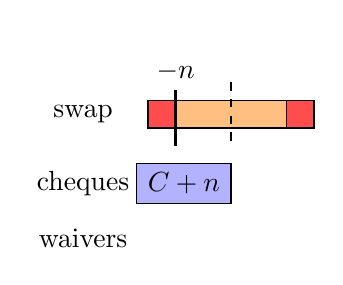
\begin{tikzpicture}
\node (middle)[draw, rectangle, fill=orange!50, minimum height=1em, minimum width=4em]{};
\node (leftred) [draw, rectangle, fill=red!70, minimum height=1em, minimum width=1em, node distance=2.5em, left of=middle]{};
\node (rightred)[draw, rectangle, fill=red!70, minimum height=1em, minimum width=1em, node distance=2.5em, right of=middle]{};
\node (zero) [above of=middle,node distance=2em, text height=1em] {};
\node (zerod) [below of=zero, node distance=3.5em] {};
\node (balance) [left of=zero,node distance=2em, text height=1.5em] {$-n$};
\node (balanced) [below of=balance,node distance=3.5em] {};
\draw [dashed](zero)--(zerod);
\draw [very thick](balance)--(balanced);
\node (payment) [below of=zerod, node distance=1em]{};
\node (cheque) [draw, left of=payment, node distance=1.7em, minimum height=1em, minimum width=3.4em, fill=blue!30, rectangle]{$C+n$};

\node (swap) [left of=leftred,minimum width=1em,align=right]{swap};
\node (cheques) [below of=swap,minimum width=1em, node distance= 2.5em, align=right]{cheques};
\node (waivers) [below of=cheques,minimum width=1em, node distance= 2em, align=right]{waivers};
\end{tikzpicture}
&
\begin{tabular}{c}
  $\Longrightarrow$
\\ \\ \\ \\
\end{tabular}
&
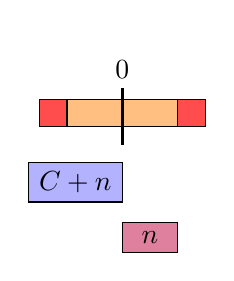
\begin{tikzpicture}
\node (middle)[draw, rectangle, fill=orange!50, minimum height=1em, minimum width=4em]{};
\node (leftred) [draw, rectangle, fill=red!70, minimum height=1em, minimum width=1em, node distance=2.5em, left of=middle]{};
\node (rightred)[draw, rectangle, fill=red!70, minimum height=1em, minimum width=1em, node distance=2.5em, right of=middle]{};
\node (zero) [above of=middle,node distance=2em, text height=1.5em] {$0$};
\node (zerod) [below of=zero, node distance=3.5em] {};
% \draw [dashed](zero)--(zerod);
\draw [very thick](zero)--(zerod);
\node (payment) [below of=zerod, node distance=1em]{};
\node (cheque) [draw, left of=payment, node distance=1.7em, minimum height=1em, minimum width=3.4em, fill=blue!30, rectangle]{$C+n$};
\node (waivers) [below of=payment, node distance=2em]{};
\node (waiver) [right of=waivers,minimum width=2em, node distance=1em,rectangle,draw,fill=purple!50]{$n$};
\end{tikzpicture}
\end{tabular}
\end{center}

\caption{Peer A's swap balance (with respect to B) reaches the payment threshold $n$ (left),
A sends a waiver to peer B. B keeps the waiver and restores the swap balance to zero}
\label{fig:waiverswap}
\end{figure}
\end{center}

